\documentclass[1p]{elsarticle_modified}
%\bibliographystyle{elsarticle-num}

%\usepackage[colorlinks]{hyperref}
%\usepackage{abbrmath_seonhwa} %\Abb, \Ascr, \Acal ,\Abf, \Afrak
\usepackage{amsfonts}
\usepackage{amssymb}
\usepackage{amsmath}
\usepackage{amsthm}
\usepackage{scalefnt}
\usepackage{amsbsy}
\usepackage{kotex}
\usepackage{caption}
\usepackage{subfig}
\usepackage{color}
\usepackage{graphicx}
\usepackage{xcolor} %% white, black, red, green, blue, cyan, magenta, yellow
\usepackage{float}
\usepackage{setspace}
\usepackage{hyperref}

\usepackage{tikz}
\usetikzlibrary{arrows}

\usepackage{multirow}
\usepackage{array} % fixed length table
\usepackage{hhline}

%%%%%%%%%%%%%%%%%%%%%
\makeatletter
\renewcommand*\env@matrix[1][\arraystretch]{%
	\edef\arraystretch{#1}%
	\hskip -\arraycolsep
	\let\@ifnextchar\new@ifnextchar
	\array{*\c@MaxMatrixCols c}}
\makeatother %https://tex.stackexchange.com/questions/14071/how-can-i-increase-the-line-spacing-in-a-matrix
%%%%%%%%%%%%%%%

\usepackage[normalem]{ulem}

\newcommand{\msout}[1]{\ifmmode\text{\sout{\ensuremath{#1}}}\else\sout{#1}\fi}
%SOURCE: \msout is \stkout macro in https://tex.stackexchange.com/questions/20609/strikeout-in-math-mode

\newcommand{\cancel}[1]{
	\ifmmode
	{\color{red}\msout{#1}}
	\else
	{\color{red}\sout{#1}}
	\fi
}

\newcommand{\add}[1]{
	{\color{blue}\uwave{#1}}
}

\newcommand{\replace}[2]{
	\ifmmode
	{\color{red}\msout{#1}}{\color{blue}\uwave{#2}}
	\else
	{\color{red}\sout{#1}}{\color{blue}\uwave{#2}}
	\fi
}

\newcommand{\Sol}{\mathcal{S}} %segment
\newcommand{\D}{D} %diagram
\newcommand{\A}{\mathcal{A}} %arc


%%%%%%%%%%%%%%%%%%%%%%%%%%%%%5 test

\def\sl{\operatorname{\textup{SL}}(2,\Cbb)}
\def\psl{\operatorname{\textup{PSL}}(2,\Cbb)}
\def\quan{\mkern 1mu \triangleright \mkern 1mu}

\theoremstyle{definition}
\newtheorem{thm}{Theorem}[section]
\newtheorem{prop}[thm]{Proposition}
\newtheorem{lem}[thm]{Lemma}
\newtheorem{ques}[thm]{Question}
\newtheorem{cor}[thm]{Corollary}
\newtheorem{defn}[thm]{Definition}
\newtheorem{exam}[thm]{Example}
\newtheorem{rmk}[thm]{Remark}
\newtheorem{alg}[thm]{Algorithm}

\newcommand{\I}{\sqrt{-1}}
\begin{document}

%\begin{frontmatter}
%
%\title{Boundary parabolic representations of knots up to 8 crossings}
%
%%% Group authors per affiliation:
%\author{Yunhi Cho} 
%\address{Department of Mathematics, University of Seoul, Seoul, Korea}
%\ead{yhcho@uos.ac.kr}
%
%
%\author{Seonhwa Kim} %\fnref{s_kim}}
%\address{Center for Geometry and Physics, Institute for Basic Science, Pohang, 37673, Korea}
%\ead{ryeona17@ibs.re.kr}
%
%\author{Hyuk Kim}
%\address{Department of Mathematical Sciences, Seoul National University, Seoul 08826, Korea}
%\ead{hyukkim@snu.ac.kr}
%
%\author{Seokbeom Yoon}
%\address{Department of Mathematical Sciences, Seoul National University, Seoul, 08826,  Korea}
%\ead{sbyoon15@snu.ac.kr}
%
%\begin{abstract}
%We find all boundary parabolic representation of knots up to 8 crossings.
%
%\end{abstract}
%\begin{keyword}
%    \MSC[2010] 57M25 
%\end{keyword}
%
%\end{frontmatter}

%\linenumbers
%\tableofcontents
%
\newcommand\colored[1]{\textcolor{white}{\rule[-0.35ex]{0.8em}{1.4ex}}\kern-0.8em\color{red} #1}%
%\newcommand\colored[1]{\textcolor{white}{ #1}\kern-2.17ex	\textcolor{white}{ #1}\kern-1.81ex	\textcolor{white}{ #1}\kern-2.15ex\color{red}#1	}

{\Large $\underline{12n_{0603}~(K12n_{0603})}$}

\setlength{\tabcolsep}{10pt}
\renewcommand{\arraystretch}{1.6}
\vspace{1cm}\begin{tabular}{m{100pt}>{\centering\arraybackslash}m{274pt}}
\multirow{5}{120pt}{
	\centering
	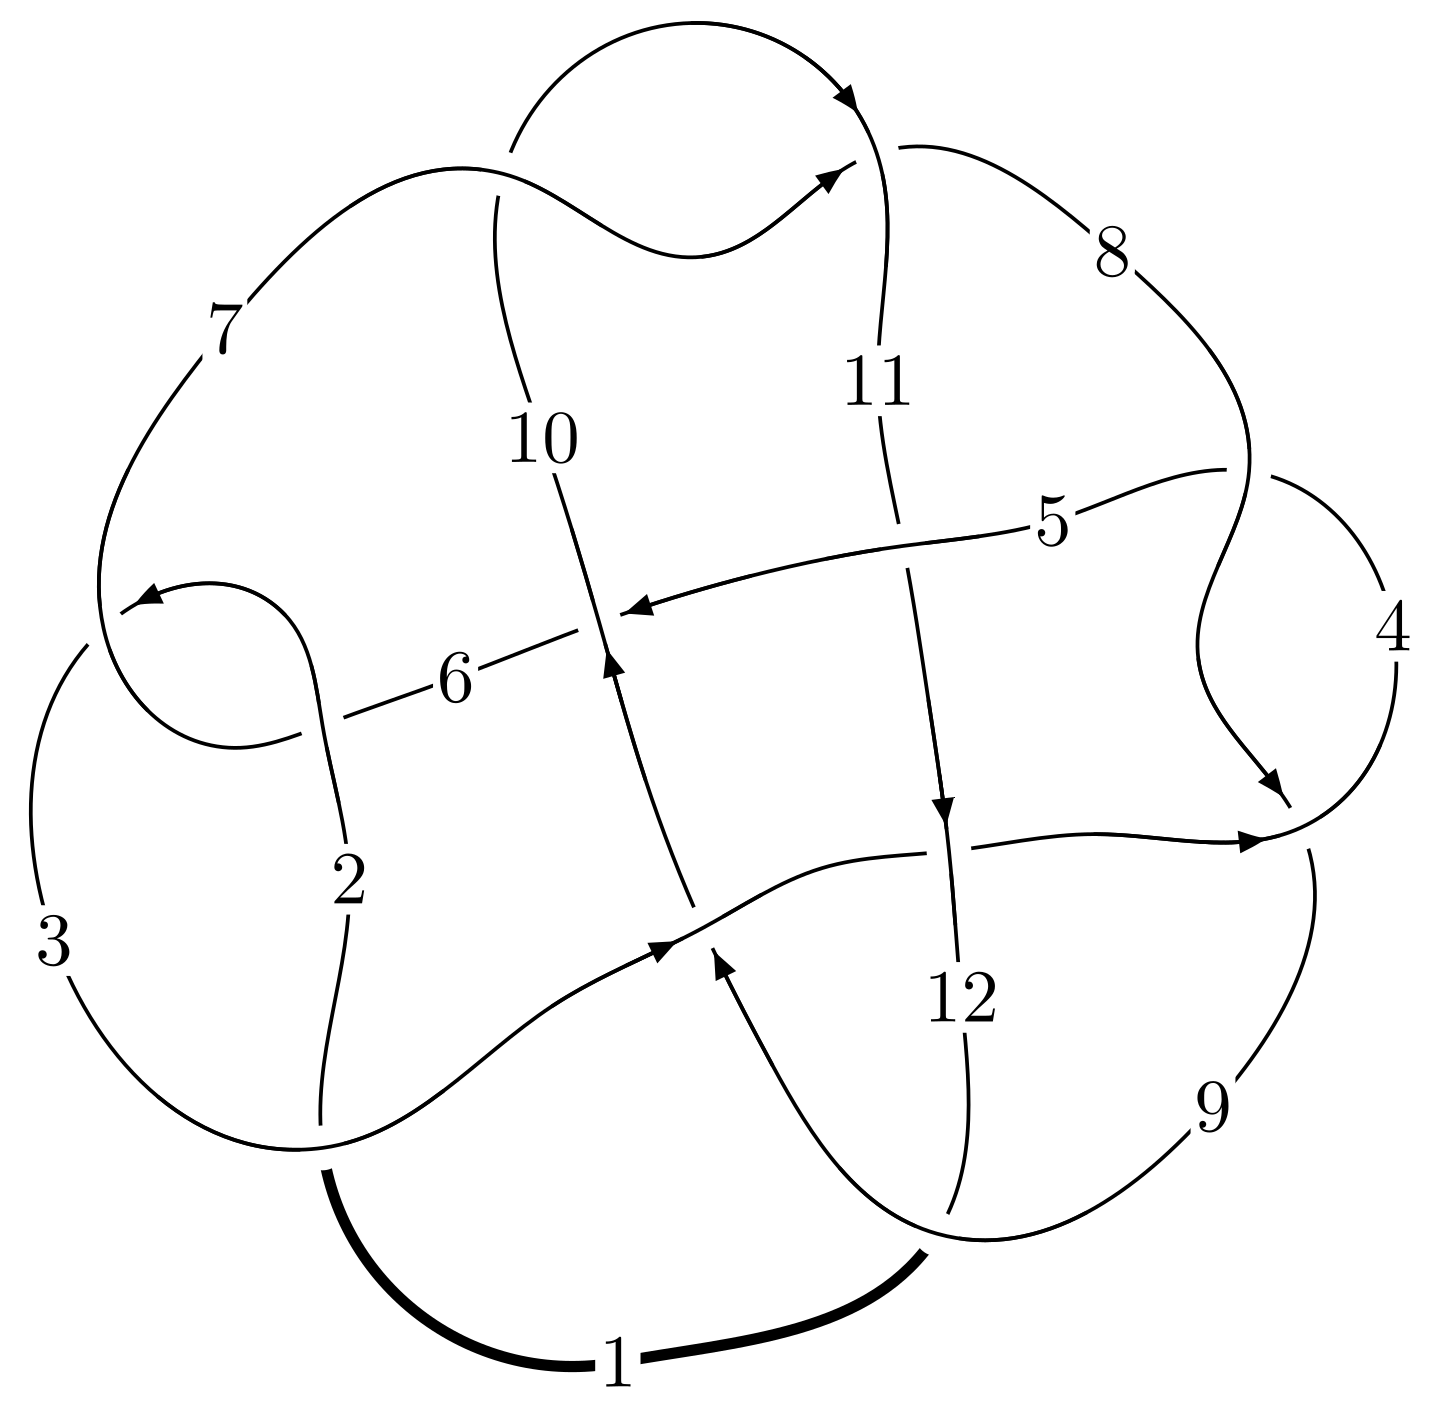
\includegraphics[width=112pt]{../../../GIT/diagram.site/Diagrams/png/2692_12n_0603.png}\\
\ \ \ A knot diagram\footnotemark}&
\allowdisplaybreaks
\textbf{Linearized knot diagam} \\
\cline{2-2}
 &
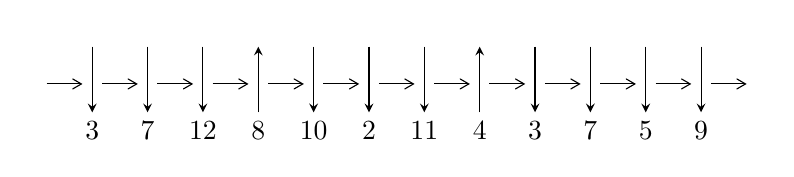
\begin{tikzpicture}[x=20pt, y=17pt]
	% nodes
	\node (C0) at (0, 0) {};
	\node (C1) at (1, 0) {};
	\node (C1U) at (1, +1) {};
	\node (C1D) at (1, -1) {3};

	\node (C2) at (2, 0) {};
	\node (C2U) at (2, +1) {};
	\node (C2D) at (2, -1) {7};

	\node (C3) at (3, 0) {};
	\node (C3U) at (3, +1) {};
	\node (C3D) at (3, -1) {12};

	\node (C4) at (4, 0) {};
	\node (C4U) at (4, +1) {};
	\node (C4D) at (4, -1) {8};

	\node (C5) at (5, 0) {};
	\node (C5U) at (5, +1) {};
	\node (C5D) at (5, -1) {10};

	\node (C6) at (6, 0) {};
	\node (C6U) at (6, +1) {};
	\node (C6D) at (6, -1) {2};

	\node (C7) at (7, 0) {};
	\node (C7U) at (7, +1) {};
	\node (C7D) at (7, -1) {11};

	\node (C8) at (8, 0) {};
	\node (C8U) at (8, +1) {};
	\node (C8D) at (8, -1) {4};

	\node (C9) at (9, 0) {};
	\node (C9U) at (9, +1) {};
	\node (C9D) at (9, -1) {3};

	\node (C10) at (10, 0) {};
	\node (C10U) at (10, +1) {};
	\node (C10D) at (10, -1) {7};

	\node (C11) at (11, 0) {};
	\node (C11U) at (11, +1) {};
	\node (C11D) at (11, -1) {5};

	\node (C12) at (12, 0) {};
	\node (C12U) at (12, +1) {};
	\node (C12D) at (12, -1) {9};
	\node (C13) at (13, 0) {};

	% arrows
	\draw[->,>={angle 60}]
	(C0) edge (C1) (C1) edge (C2) (C2) edge (C3) (C3) edge (C4) (C4) edge (C5) (C5) edge (C6) (C6) edge (C7) (C7) edge (C8) (C8) edge (C9) (C9) edge (C10) (C10) edge (C11) (C11) edge (C12) (C12) edge (C13) ;	\draw[->,>=stealth]
	(C1U) edge (C1D) (C2U) edge (C2D) (C3U) edge (C3D) (C4D) edge (C4U) (C5U) edge (C5D) (C6U) edge (C6D) (C7U) edge (C7D) (C8D) edge (C8U) (C9U) edge (C9D) (C10U) edge (C10D) (C11U) edge (C11D) (C12U) edge (C12D) ;
	\end{tikzpicture} \\
\hhline{~~} \\& 
\textbf{Solving Sequence} \\ \cline{2-2} 
 &
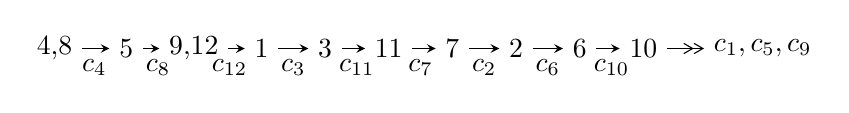
\begin{tikzpicture}[x=23pt, y=7pt]
	% node
	\node (A0) at (-1/8, 0) {4,8};
	\node (A1) at (1, 0) {5};
	\node (A2) at (33/16, 0) {9,12};
	\node (A3) at (25/8, 0) {1};
	\node (A4) at (33/8, 0) {3};
	\node (A5) at (41/8, 0) {11};
	\node (A6) at (49/8, 0) {7};
	\node (A7) at (57/8, 0) {2};
	\node (A8) at (65/8, 0) {6};
	\node (A9) at (73/8, 0) {10};
	\node (C1) at (1/2, -1) {$c_{4}$};
	\node (C2) at (3/2, -1) {$c_{8}$};
	\node (C3) at (21/8, -1) {$c_{12}$};
	\node (C4) at (29/8, -1) {$c_{3}$};
	\node (C5) at (37/8, -1) {$c_{11}$};
	\node (C6) at (45/8, -1) {$c_{7}$};
	\node (C7) at (53/8, -1) {$c_{2}$};
	\node (C8) at (61/8, -1) {$c_{6}$};
	\node (C9) at (69/8, -1) {$c_{10}$};
	\node (A10) at (11, 0) {$c_{1},c_{5},c_{9}$};

	% edge
	\draw[->,>=stealth]	
	(A0) edge (A1) (A1) edge (A2) (A2) edge (A3) (A3) edge (A4) (A4) edge (A5) (A5) edge (A6) (A6) edge (A7) (A7) edge (A8) (A8) edge (A9) ;
	\draw[->>,>={angle 60}]	
	(A9) edge (A10);
\end{tikzpicture} \\ 

\end{tabular} \\

\footnotetext{
The image of knot diagram is generated by the software ``\textbf{Draw programme}" developed by Andrew Bartholomew(\url{http://www.layer8.co.uk/maths/draw/index.htm\#Running-draw}), where we modified some parts for our purpose(\url{https://github.com/CATsTAILs/LinksPainter}).
}\phantom \\ \newline 
\centering \textbf{Ideals for irreducible components\footnotemark of $X_{\text{par}}$} 
 
\begin{align*}
I^u_{1}&=\langle 
478 u^{12}+178 u^{11}+\cdots+122 b-1078,\;a-1,\\
\phantom{I^u_{1}}&\phantom{= \langle  }u^{13}+8 u^{11}+3 u^{10}+25 u^9+18 u^8+32 u^7+33 u^6+10 u^5+14 u^4- u^3-10 u^2+1\rangle \\
I^u_{2}&=\langle 
2 u^9+7 u^7+4 u^6+7 u^5+10 u^4-6 u^3+7 u^2+2 b-8 u+2,\;a+1,\\
\phantom{I^u_{2}}&\phantom{= \langle  }u^{10}+4 u^8+2 u^7+5 u^6+6 u^5-2 u^4+6 u^3-6 u^2+2 u-1\rangle \\
I^u_{3}&=\langle 
u^5-3 u^4+7 u^3-16 u^2+9 b+8 u-10,\;-19 u^5+39 u^4-79 u^3+178 u^2+9 a-35 u+226,\\
\phantom{I^u_{3}}&\phantom{= \langle  }u^6-2 u^5+4 u^4-9 u^3+u^2-11 u-1\rangle \\
I^u_{4}&=\langle 
b,\;a- u,\;u^2- u+1\rangle \\
\\
\end{align*}
\raggedright * 4 irreducible components of $\dim_{\mathbb{C}}=0$, with total 31 representations.\\
\footnotetext{All coefficients of polynomials are rational numbers. But the coefficients are sometimes approximated in decimal forms when there is not enough margin.}
\newpage
\renewcommand{\arraystretch}{1}
\centering \section*{I. $I^u_{1}= \langle 478 u^{12}+178 u^{11}+\cdots+122 b-1078,\;a-1,\;u^{13}+8 u^{11}+\cdots-10 u^2+1 \rangle$}
\flushleft \textbf{(i) Arc colorings}\\
\begin{tabular}{m{7pt} m{180pt} m{7pt} m{180pt} }
\flushright $a_{4}=$&$\begin{pmatrix}1\\0\end{pmatrix}$ \\
\flushright $a_{8}=$&$\begin{pmatrix}0\\u\end{pmatrix}$ \\
\flushright $a_{5}=$&$\begin{pmatrix}1\\- u^2\end{pmatrix}$ \\
\flushright $a_{9}=$&$\begin{pmatrix}u\\u\end{pmatrix}$ \\
\flushright $a_{12}=$&$\begin{pmatrix}1\\-3.91803 u^{12}-1.45902 u^{11}+\cdots+23.6721 u+8.83607\end{pmatrix}$ \\
\flushright $a_{1}=$&$\begin{pmatrix}0.729508 u^{12}+0.114754 u^{11}+\cdots-3.91803 u-0.459016\\-3.18852 u^{12}-1.34426 u^{11}+\cdots+19.7541 u+7.37705\end{pmatrix}$ \\
\flushright $a_{3}=$&$\begin{pmatrix}3.91803 u^{12}+1.45902 u^{11}+\cdots-23.6721 u-7.83607\\-2.60656 u^{12}-0.803279 u^{11}+\cdots+16.9262 u+6.21311\end{pmatrix}$ \\
\flushright $a_{11}=$&$\begin{pmatrix}-3.91803 u^{12}-1.45902 u^{11}+\cdots+23.6721 u+9.83607\\-3.18852 u^{12}-1.34426 u^{11}+\cdots+19.7541 u+7.37705\end{pmatrix}$ \\
\flushright $a_{7}=$&$\begin{pmatrix}-2.34426 u^{12}-1.17213 u^{11}+\cdots+15.3770 u+6.68852\\-0.549180 u^{12}-0.0245902 u^{11}+\cdots+4.19672 u+1.59836\end{pmatrix}$ \\
\flushright $a_{2}=$&$\begin{pmatrix}6.62295 u^{12}+2.81148 u^{11}+\cdots-40.4918 u-14.7459\\-1.68852 u^{12}+0.155738 u^{11}+\cdots+12.2541 u+4.37705\end{pmatrix}$ \\
\flushright $a_{6}=$&$\begin{pmatrix}5.24590 u^{12}+1.12295 u^{11}+\cdots-29.9836 u-12.9918\\-0.655738 u^{12}-2.32787 u^{11}+\cdots+3.62295 u+0.311475\end{pmatrix}$ \\
\flushright $a_{10}=$&$\begin{pmatrix}-3.07377 u^{12}-1.28689 u^{11}+\cdots+20.2951 u+9.14754\\-3.12295 u^{12}-0.811475 u^{11}+\cdots+19.9918 u+7.74590\end{pmatrix}$\\&\end{tabular}
\flushleft \textbf{(ii) Obstruction class $= -1$}\\~\\
\flushleft \textbf{(iii) Cusp Shapes $= \frac{125}{122} u^{12}+\frac{215}{122} u^{11}+\frac{1077}{122} u^{10}+\frac{1082}{61} u^9+\frac{4329}{122} u^8+\frac{4205}{61} u^7+\frac{4804}{61} u^6+\frac{6996}{61} u^5+\frac{11113}{122} u^4+\frac{8069}{122} u^3+\frac{2702}{61} u^2-\frac{6}{61} u-\frac{979}{61}$}\\~\\
\newpage\renewcommand{\arraystretch}{1}
\flushleft \textbf{(iv) u-Polynomials at the component}\newline \\
\begin{tabular}{m{50pt}|m{274pt}}
Crossings & \hspace{64pt}u-Polynomials at each crossing \\
\hline $$\begin{aligned}c_{1}\end{aligned}$$&$\begin{aligned}
&u^{13}+32 u^{12}+\cdots+33 u+1
\end{aligned}$\\
\hline $$\begin{aligned}c_{2},c_{6}\end{aligned}$$&$\begin{aligned}
&u^{13}-2 u^{12}+\cdots-5 u+1
\end{aligned}$\\
\hline $$\begin{aligned}c_{3}\end{aligned}$$&$\begin{aligned}
&u^{13}-8 u^{12}+\cdots-9 u+2
\end{aligned}$\\
\hline $$\begin{aligned}c_{4},c_{8}\end{aligned}$$&$\begin{aligned}
&u^{13}+8 u^{11}+\cdots-10 u^2+1
\end{aligned}$\\
\hline $$\begin{aligned}c_{5}\end{aligned}$$&$\begin{aligned}
&u^{13}-25 u^{12}+\cdots+9173 u+2591
\end{aligned}$\\
\hline $$\begin{aligned}c_{7},c_{10}\end{aligned}$$&$\begin{aligned}
&u^{13}+8 u^{12}+\cdots+27 u+4
\end{aligned}$\\
\hline $$\begin{aligned}c_{9}\end{aligned}$$&$\begin{aligned}
&u^{13}-18 u^{11}+\cdots+738 u+244
\end{aligned}$\\
\hline $$\begin{aligned}c_{11}\end{aligned}$$&$\begin{aligned}
&u^{13}+8 u^{12}+\cdots+20 u+4
\end{aligned}$\\
\hline $$\begin{aligned}c_{12}\end{aligned}$$&$\begin{aligned}
&u^{13}+u^{12}+\cdots+u+1
\end{aligned}$\\
\hline
\end{tabular}\\~\\
\newpage\renewcommand{\arraystretch}{1}
\flushleft \textbf{(v) Riley Polynomials at the component}\newline \\
\begin{tabular}{m{50pt}|m{274pt}}
Crossings & \hspace{64pt}Riley Polynomials at each crossing \\
\hline $$\begin{aligned}c_{1}\end{aligned}$$&$\begin{aligned}
&y^{13}-308 y^{12}+\cdots+249 y-1
\end{aligned}$\\
\hline $$\begin{aligned}c_{2},c_{6}\end{aligned}$$&$\begin{aligned}
&y^{13}-32 y^{12}+\cdots+33 y-1
\end{aligned}$\\
\hline $$\begin{aligned}c_{3}\end{aligned}$$&$\begin{aligned}
&y^{13}+24 y^{11}+\cdots+25 y-4
\end{aligned}$\\
\hline $$\begin{aligned}c_{4},c_{8}\end{aligned}$$&$\begin{aligned}
&y^{13}+16 y^{12}+\cdots+20 y-1
\end{aligned}$\\
\hline $$\begin{aligned}c_{5}\end{aligned}$$&$\begin{aligned}
&y^{13}-137 y^{12}+\cdots+11823937 y-6713281
\end{aligned}$\\
\hline $$\begin{aligned}c_{7},c_{10}\end{aligned}$$&$\begin{aligned}
&y^{13}-28 y^{12}+\cdots+345 y-16
\end{aligned}$\\
\hline $$\begin{aligned}c_{9}\end{aligned}$$&$\begin{aligned}
&y^{13}-36 y^{12}+\cdots-302036 y-59536
\end{aligned}$\\
\hline $$\begin{aligned}c_{11}\end{aligned}$$&$\begin{aligned}
&y^{13}+2 y^{12}+\cdots+120 y-16
\end{aligned}$\\
\hline $$\begin{aligned}c_{12}\end{aligned}$$&$\begin{aligned}
&y^{13}-25 y^{12}+\cdots-7 y-1
\end{aligned}$\\
\hline
\end{tabular}\\~\\
\newpage\flushleft \textbf{(vi) Complex Volumes and Cusp Shapes}
$$\begin{array}{c|c|c}  
\text{Solutions to }I^u_{1}& \I (\text{vol} + \sqrt{-1}CS) & \text{Cusp shape}\\
 \hline 
\begin{aligned}
u &= \phantom{-}0.231299 + 1.092720 I \\
a &= \phantom{-}1.00000\phantom{ +0.000000I} \\
b &= \phantom{-}0.502972 - 0.016598 I\end{aligned}
 & -0.96921 + 1.60705 I & -6.76099 - 3.52286 I \\ \hline\begin{aligned}
u &= \phantom{-}0.231299 - 1.092720 I \\
a &= \phantom{-}1.00000\phantom{ +0.000000I} \\
b &= \phantom{-}0.502972 + 0.016598 I\end{aligned}
 & -0.96921 - 1.60705 I & -6.76099 + 3.52286 I \\ \hline\begin{aligned}
u &= -0.755051 + 0.130841 I \\
a &= \phantom{-}1.00000\phantom{ +0.000000I} \\
b &= \phantom{-}0.012282 + 0.611071 I\end{aligned}
 & -1.91994 - 0.62113 I & -7.84819 + 2.13633 I \\ \hline\begin{aligned}
u &= -0.755051 - 0.130841 I \\
a &= \phantom{-}1.00000\phantom{ +0.000000I} \\
b &= \phantom{-}0.012282 - 0.611071 I\end{aligned}
 & -1.91994 + 0.62113 I & -7.84819 - 2.13633 I \\ \hline\begin{aligned}
u &= -0.06382 + 1.54550 I \\
a &= \phantom{-}1.00000\phantom{ +0.000000I} \\
b &= \phantom{-}1.25006 + 1.58656 I\end{aligned}
 & \phantom{-}15.3034 - 0.5963 I & -12.36984 + 0.02697 I \\ \hline\begin{aligned}
u &= -0.06382 - 1.54550 I \\
a &= \phantom{-}1.00000\phantom{ +0.000000I} \\
b &= \phantom{-}1.25006 - 1.58656 I\end{aligned}
 & \phantom{-}15.3034 + 0.5963 I & -12.36984 - 0.02697 I \\ \hline\begin{aligned}
u &= \phantom{-}0.404295 + 0.009197 I \\
a &= \phantom{-}1.00000\phantom{ +0.000000I} \\
b &= -0.308660 - 1.174280 I\end{aligned}
 & \phantom{-}2.44055 - 2.02483 I & -0.337255 + 1.060894 I \\ \hline\begin{aligned}
u &= \phantom{-}0.404295 - 0.009197 I \\
a &= \phantom{-}1.00000\phantom{ +0.000000I} \\
b &= -0.308660 + 1.174280 I\end{aligned}
 & \phantom{-}2.44055 + 2.02483 I & -0.337255 - 1.060894 I \\ \hline\begin{aligned}
u &= -0.31241 + 1.60855 I \\
a &= \phantom{-}1.00000\phantom{ +0.000000I} \\
b &= \phantom{-}1.354220 - 0.086669 I\end{aligned}
 & -8.31754 - 4.12811 I & -12.63192 + 2.04182 I \\ \hline\begin{aligned}
u &= -0.31241 - 1.60855 I \\
a &= \phantom{-}1.00000\phantom{ +0.000000I} \\
b &= \phantom{-}1.354220 + 0.086669 I\end{aligned}
 & -8.31754 + 4.12811 I & -12.63192 - 2.04182 I\\
 \hline 
 \end{array}$$\newpage$$\begin{array}{c|c|c}  
\text{Solutions to }I^u_{1}& \I (\text{vol} + \sqrt{-1}CS) & \text{Cusp shape}\\
 \hline 
\begin{aligned}
u &= -0.354088\phantom{ +0.000000I} \\
a &= \phantom{-}1.00000\phantom{ +0.000000I} \\
b &= -0.507588\phantom{ +0.000000I}\end{aligned}
 & -0.805953\phantom{ +0.000000I} & -12.4890\phantom{ +0.000000I} \\ \hline\begin{aligned}
u &= \phantom{-}0.67274 + 1.79353 I \\
a &= \phantom{-}1.00000\phantom{ +0.000000I} \\
b &= \phantom{-}1.44292 - 1.29558 I\end{aligned}
 & \phantom{-}14.4274 + 9.8229 I & -12.30738 - 3.83207 I \\ \hline\begin{aligned}
u &= \phantom{-}0.67274 - 1.79353 I \\
a &= \phantom{-}1.00000\phantom{ +0.000000I} \\
b &= \phantom{-}1.44292 + 1.29558 I\end{aligned}
 & \phantom{-}14.4274 - 9.8229 I & -12.30738 + 3.83207 I\\
 \hline 
 \end{array}$$\newpage\newpage\renewcommand{\arraystretch}{1}
\centering \section*{II. $I^u_{2}= \langle 2 u^9+7 u^7+\cdots+2 b+2,\;a+1,\;u^{10}+4 u^8+\cdots+2 u-1 \rangle$}
\flushleft \textbf{(i) Arc colorings}\\
\begin{tabular}{m{7pt} m{180pt} m{7pt} m{180pt} }
\flushright $a_{4}=$&$\begin{pmatrix}1\\0\end{pmatrix}$ \\
\flushright $a_{8}=$&$\begin{pmatrix}0\\u\end{pmatrix}$ \\
\flushright $a_{5}=$&$\begin{pmatrix}1\\- u^2\end{pmatrix}$ \\
\flushright $a_{9}=$&$\begin{pmatrix}u\\u\end{pmatrix}$ \\
\flushright $a_{12}=$&$\begin{pmatrix}-1\\- u^9-\frac{7}{2} u^7+\cdots+4 u-1\end{pmatrix}$ \\
\flushright $a_{1}=$&$\begin{pmatrix}-\frac{1}{2} u^9-\frac{3}{2} u^7+\cdots+u-1\\-\frac{3}{2} u^9-5 u^7+\cdots+5 u-1\end{pmatrix}$ \\
\flushright $a_{3}=$&$\begin{pmatrix}- u^9-\frac{7}{2} u^7+\cdots-\frac{7}{2} u^2+4 u\\- u^9-\frac{7}{2} u^7+\cdots+\frac{5}{2} u+1\end{pmatrix}$ \\
\flushright $a_{11}=$&$\begin{pmatrix}- u^9-\frac{7}{2} u^7+\cdots+4 u-2\\-\frac{3}{2} u^9-5 u^7+\cdots+5 u-1\end{pmatrix}$ \\
\flushright $a_{7}=$&$\begin{pmatrix}-\frac{1}{2} u^8+\frac{1}{2} u^7+\cdots-2 u+2\\-\frac{1}{2} u^9-\frac{1}{2} u^8+\cdots-2 u+\frac{3}{2}\end{pmatrix}$ \\
\flushright $a_{2}=$&$\begin{pmatrix}- u^9-\frac{1}{2} u^8+\cdots-\frac{3}{2} u^2+\frac{3}{2}\\- u^9-\frac{1}{2} u^8+\cdots-\frac{1}{2} u+2\end{pmatrix}$ \\
\flushright $a_{6}=$&$\begin{pmatrix}\frac{1}{2} u^8-\frac{1}{2} u^7+\cdots+u-\frac{1}{2}\\u^5- u^4+4 u^3-3 u^2+4 u-2\end{pmatrix}$ \\
\flushright $a_{10}=$&$\begin{pmatrix}-\frac{1}{2} u^9+\frac{1}{2} u^8+\cdots+4 u-1\\-\frac{1}{2} u^9+\frac{1}{2} u^8+\cdots+\frac{9}{2} u-\frac{1}{2}\end{pmatrix}$\\&\end{tabular}
\flushleft \textbf{(ii) Obstruction class $= 1$}\\~\\
\flushleft \textbf{(iii) Cusp Shapes $= \frac{5}{2} u^9-\frac{1}{2} u^8+\frac{19}{2} u^7+\frac{7}{2} u^6+9 u^5+\frac{27}{2} u^4-\frac{21}{2} u^3+12 u^2-16 u-10$}\\~\\
\newpage\renewcommand{\arraystretch}{1}
\flushleft \textbf{(iv) u-Polynomials at the component}\newline \\
\begin{tabular}{m{50pt}|m{274pt}}
Crossings & \hspace{64pt}u-Polynomials at each crossing \\
\hline $$\begin{aligned}c_{1}\end{aligned}$$&$\begin{aligned}
&u^{10}-12 u^9+38 u^8-81 u^7+109 u^6-102 u^5+62 u^4-18 u^3- u+1
\end{aligned}$\\
\hline $$\begin{aligned}c_{2}\end{aligned}$$&$\begin{aligned}
&u^{10}-2 u^9-4 u^8+3 u^7+5 u^6-6 u^5-4 u^4+4 u^3- u+1
\end{aligned}$\\
\hline $$\begin{aligned}c_{3}\end{aligned}$$&$\begin{aligned}
&u^{10}+5 u^9+\cdots-15 u-3
\end{aligned}$\\
\hline $$\begin{aligned}c_{4}\end{aligned}$$&$\begin{aligned}
&u^{10}+4 u^8+2 u^7+5 u^6+6 u^5-2 u^4+6 u^3-6 u^2+2 u-1
\end{aligned}$\\
\hline $$\begin{aligned}c_{5}\end{aligned}$$&$\begin{aligned}
&u^{10}-3 u^9-10 u^8-6 u^7-8 u^6-18 u^5+7 u^3+8 u^2+3 u+1
\end{aligned}$\\
\hline $$\begin{aligned}c_{6}\end{aligned}$$&$\begin{aligned}
&u^{10}+2 u^9-4 u^8-3 u^7+5 u^6+6 u^5-4 u^4-4 u^3+u+1
\end{aligned}$\\
\hline $$\begin{aligned}c_{7}\end{aligned}$$&$\begin{aligned}
&u^{10}+5 u^9+6 u^8-5 u^7-10 u^6+2 u^5-6 u^3+6 u^2+3 u-5
\end{aligned}$\\
\hline $$\begin{aligned}c_{8}\end{aligned}$$&$\begin{aligned}
&u^{10}+4 u^8-2 u^7+5 u^6-6 u^5-2 u^4-6 u^3-6 u^2-2 u-1
\end{aligned}$\\
\hline $$\begin{aligned}c_{9}\end{aligned}$$&$\begin{aligned}
&u^{10}-5 u^9+5 u^8+u^7-9 u^6+6 u^5-3 u^4-7 u^3+3 u^2-1
\end{aligned}$\\
\hline $$\begin{aligned}c_{10}\end{aligned}$$&$\begin{aligned}
&u^{10}-5 u^9+6 u^8+5 u^7-10 u^6-2 u^5+6 u^3+6 u^2-3 u-5
\end{aligned}$\\
\hline $$\begin{aligned}c_{11}\end{aligned}$$&$\begin{aligned}
&u^{10}+3 u^9+6 u^8+6 u^7+4 u^6-2 u^5-5 u^4-7 u^3+2 u+1
\end{aligned}$\\
\hline $$\begin{aligned}c_{12}\end{aligned}$$&$\begin{aligned}
&u^{10}- u^9-6 u^8+3 u^7+11 u^6-9 u^5-11 u^4+5 u^3+2 u^2-3 u-1
\end{aligned}$\\
\hline
\end{tabular}\\~\\
\newpage\renewcommand{\arraystretch}{1}
\flushleft \textbf{(v) Riley Polynomials at the component}\newline \\
\begin{tabular}{m{50pt}|m{274pt}}
Crossings & \hspace{64pt}Riley Polynomials at each crossing \\
\hline $$\begin{aligned}c_{1}\end{aligned}$$&$\begin{aligned}
&y^{10}-68 y^9+\cdots- y+1
\end{aligned}$\\
\hline $$\begin{aligned}c_{2},c_{6}\end{aligned}$$&$\begin{aligned}
&y^{10}-12 y^9+38 y^8-81 y^7+109 y^6-102 y^5+62 y^4-18 y^3- y+1
\end{aligned}$\\
\hline $$\begin{aligned}c_{3}\end{aligned}$$&$\begin{aligned}
&y^{10}+3 y^9+4 y^8+3 y^7+9 y^6+15 y^5+9 y^4- y^3+16 y^2-57 y+9
\end{aligned}$\\
\hline $$\begin{aligned}c_{4},c_{8}\end{aligned}$$&$\begin{aligned}
&y^{10}+8 y^9+\cdots+8 y+1
\end{aligned}$\\
\hline $$\begin{aligned}c_{5}\end{aligned}$$&$\begin{aligned}
&y^{10}-29 y^9+\cdots+7 y+1
\end{aligned}$\\
\hline $$\begin{aligned}c_{7},c_{10}\end{aligned}$$&$\begin{aligned}
&y^{10}-13 y^9+\cdots-69 y+25
\end{aligned}$\\
\hline $$\begin{aligned}c_{9}\end{aligned}$$&$\begin{aligned}
&y^{10}-15 y^9+\cdots-6 y+1
\end{aligned}$\\
\hline $$\begin{aligned}c_{11}\end{aligned}$$&$\begin{aligned}
&y^{10}+3 y^9+8 y^8+14 y^7+22 y^6+30 y^5-15 y^4-33 y^3+18 y^2-4 y+1
\end{aligned}$\\
\hline $$\begin{aligned}c_{12}\end{aligned}$$&$\begin{aligned}
&y^{10}-13 y^9+\cdots-13 y+1
\end{aligned}$\\
\hline
\end{tabular}\\~\\
\newpage\flushleft \textbf{(vi) Complex Volumes and Cusp Shapes}
$$\begin{array}{c|c|c}  
\text{Solutions to }I^u_{2}& \I (\text{vol} + \sqrt{-1}CS) & \text{Cusp shape}\\
 \hline 
\begin{aligned}
u &= \phantom{-}0.009496 + 1.155230 I \\
a &= -1.00000\phantom{ +0.000000I} \\
b &= -0.572116 - 1.276800 I\end{aligned}
 & -5.38125 + 0.86206 I & -11.68799 - 0.71640 I \\ \hline\begin{aligned}
u &= \phantom{-}0.009496 - 1.155230 I \\
a &= -1.00000\phantom{ +0.000000I} \\
b &= -0.572116 + 1.276800 I\end{aligned}
 & -5.38125 - 0.86206 I & -11.68799 + 0.71640 I \\ \hline\begin{aligned}
u &= -1.28347\phantom{ +0.000000I} \\
a &= -1.00000\phantom{ +0.000000I} \\
b &= \phantom{-}0.970806\phantom{ +0.000000I}\end{aligned}
 & -17.3343\phantom{ +0.000000I} & -8.37670\phantom{ +0.000000I} \\ \hline\begin{aligned}
u &= -0.335045 + 1.275960 I \\
a &= -1.00000\phantom{ +0.000000I} \\
b &= -1.122050 - 0.534600 I\end{aligned}
 & -2.32585 - 2.89091 I & -9.34725 + 3.73381 I \\ \hline\begin{aligned}
u &= -0.335045 - 1.275960 I \\
a &= -1.00000\phantom{ +0.000000I} \\
b &= -1.122050 + 0.534600 I\end{aligned}
 & -2.32585 + 2.89091 I & -9.34725 - 3.73381 I \\ \hline\begin{aligned}
u &= \phantom{-}0.612033\phantom{ +0.000000I} \\
a &= -1.00000\phantom{ +0.000000I} \\
b &= -0.407032\phantom{ +0.000000I}\end{aligned}
 & -3.00050\phantom{ +0.000000I} & -14.5280\phantom{ +0.000000I} \\ \hline\begin{aligned}
u &= \phantom{-}0.116511 + 0.447058 I \\
a &= -1.00000\phantom{ +0.000000I} \\
b &= -0.261046 + 1.360630 I\end{aligned}
 & \phantom{-}1.90106 + 2.27397 I & -12.92039 - 5.58214 I \\ \hline\begin{aligned}
u &= \phantom{-}0.116511 - 0.447058 I \\
a &= -1.00000\phantom{ +0.000000I} \\
b &= -0.261046 - 1.360630 I\end{aligned}
 & \phantom{-}1.90106 - 2.27397 I & -12.92039 + 5.58214 I \\ \hline\begin{aligned}
u &= \phantom{-}0.54476 + 1.50703 I \\
a &= -1.00000\phantom{ +0.000000I} \\
b &= -0.826677 + 0.790310 I\end{aligned}
 & -7.05562 + 6.53270 I & -11.09214 - 5.33385 I \\ \hline\begin{aligned}
u &= \phantom{-}0.54476 - 1.50703 I \\
a &= -1.00000\phantom{ +0.000000I} \\
b &= -0.826677 - 0.790310 I\end{aligned}
 & -7.05562 - 6.53270 I & -11.09214 + 5.33385 I\\
 \hline 
 \end{array}$$\newpage\newpage\renewcommand{\arraystretch}{1}
\centering \section*{III. $I^u_{3}= \langle u^5-3 u^4+7 u^3-16 u^2+9 b+8 u-10,\;-19 u^5+39 u^4+\cdots+9 a+226,\;u^6-2 u^5+4 u^4-9 u^3+u^2-11 u-1 \rangle$}
\flushleft \textbf{(i) Arc colorings}\\
\begin{tabular}{m{7pt} m{180pt} m{7pt} m{180pt} }
\flushright $a_{4}=$&$\begin{pmatrix}1\\0\end{pmatrix}$ \\
\flushright $a_{8}=$&$\begin{pmatrix}0\\u\end{pmatrix}$ \\
\flushright $a_{5}=$&$\begin{pmatrix}1\\- u^2\end{pmatrix}$ \\
\flushright $a_{9}=$&$\begin{pmatrix}u\\u\end{pmatrix}$ \\
\flushright $a_{12}=$&$\begin{pmatrix}\frac{19}{9} u^5-\frac{13}{3} u^4+\cdots+\frac{35}{9} u-\frac{226}{9}\\-\frac{1}{9} u^5+\frac{1}{3} u^4+\cdots-\frac{8}{9} u+\frac{10}{9}\end{pmatrix}$ \\
\flushright $a_{1}=$&$\begin{pmatrix}\frac{7}{3} u^5-5 u^4+\cdots+\frac{11}{3} u-\frac{76}{3}\\\frac{1}{9} u^5-\frac{1}{3} u^4+\cdots-\frac{10}{9} u+\frac{8}{9}\end{pmatrix}$ \\
\flushright $a_{3}=$&$\begin{pmatrix}-\frac{25}{9} u^5+6 u^4+\cdots-\frac{56}{9} u+\frac{280}{9}\\\frac{2}{9} u^5-\frac{1}{3} u^4+\cdots-\frac{11}{9} u-\frac{14}{9}\end{pmatrix}$ \\
\flushright $a_{11}=$&$\begin{pmatrix}\frac{19}{9} u^5-\frac{13}{3} u^4+\cdots+\frac{35}{9} u-\frac{217}{9}\\-\frac{1}{9} u^5+\frac{1}{3} u^4+\cdots-\frac{8}{9} u+\frac{10}{9}\end{pmatrix}$ \\
\flushright $a_{7}=$&$\begin{pmatrix}\frac{43}{9} u^5-10 u^4+\cdots+\frac{83}{9} u-\frac{478}{9}\\-\frac{2}{9} u^5+\frac{1}{3} u^4+\cdots+\frac{2}{9} u+\frac{23}{9}\end{pmatrix}$ \\
\flushright $a_{2}=$&$\begin{pmatrix}-\frac{43}{3} u^5+\frac{91}{3} u^4+\cdots-\frac{83}{3} u+161\\\frac{8}{9} u^5-\frac{5}{3} u^4+\cdots-\frac{26}{9} u-\frac{71}{9}\end{pmatrix}$ \\
\flushright $a_{6}=$&$\begin{pmatrix}-30.7778 u^{5}+63.6667 u^{4}+\cdots-57.2222 u+340.444\\2 u^5-\frac{11}{3} u^4+\cdots+9 u-\frac{46}{3}\end{pmatrix}$ \\
\flushright $a_{10}=$&$\begin{pmatrix}-8.44444 u^{5}+17.6667 u^{4}+\cdots-15.5556 u+93.1111\\\frac{4}{9} u^5-\frac{1}{3} u^4+\cdots-\frac{4}{9} u-\frac{40}{9}\end{pmatrix}$\\&\end{tabular}
\flushleft \textbf{(ii) Obstruction class $= -1$}\\~\\
\flushleft \textbf{(iii) Cusp Shapes $= -\frac{1}{9} u^5+\frac{5}{9} u^3-\frac{8}{9} u^2+\frac{19}{9} u-\frac{149}{9}$}\\~\\
\newpage\renewcommand{\arraystretch}{1}
\flushleft \textbf{(iv) u-Polynomials at the component}\newline \\
\begin{tabular}{m{50pt}|m{274pt}}
Crossings & \hspace{64pt}u-Polynomials at each crossing \\
\hline $$\begin{aligned}c_{1}\end{aligned}$$&$\begin{aligned}
&u^6+23 u^5+149 u^4+597 u^3+2195 u^2+1982 u+529
\end{aligned}$\\
\hline $$\begin{aligned}c_{2},c_{6}\end{aligned}$$&$\begin{aligned}
&u^6+3 u^5-7 u^4-19 u^3-7 u^2+48 u-23
\end{aligned}$\\
\hline $$\begin{aligned}c_{3}\end{aligned}$$&$\begin{aligned}
&(u^3+u^2- u-2)^2
\end{aligned}$\\
\hline $$\begin{aligned}c_{4},c_{8}\end{aligned}$$&$\begin{aligned}
&u^6-2 u^5+4 u^4-9 u^3+u^2-11 u-1
\end{aligned}$\\
\hline $$\begin{aligned}c_{5}\end{aligned}$$&$\begin{aligned}
&u^6+6 u^5-36 u^4-47 u^3+329 u^2-331 u+101
\end{aligned}$\\
\hline $$\begin{aligned}c_{7},c_{10}\end{aligned}$$&$\begin{aligned}
&(u^3-2 u^2-1)^2
\end{aligned}$\\
\hline $$\begin{aligned}c_{9}\end{aligned}$$&$\begin{aligned}
&u^6-5 u^5-9 u^4+42 u^3-53 u^2-165 u-83
\end{aligned}$\\
\hline $$\begin{aligned}c_{11}\end{aligned}$$&$\begin{aligned}
&(u-1)^6
\end{aligned}$\\
\hline $$\begin{aligned}c_{12}\end{aligned}$$&$\begin{aligned}
&u^6-8 u^4+3 u^3+9 u^2- u-17
\end{aligned}$\\
\hline
\end{tabular}\\~\\
\newpage\renewcommand{\arraystretch}{1}
\flushleft \textbf{(v) Riley Polynomials at the component}\newline \\
\begin{tabular}{m{50pt}|m{274pt}}
Crossings & \hspace{64pt}Riley Polynomials at each crossing \\
\hline $$\begin{aligned}c_{1}\end{aligned}$$&$\begin{aligned}
&y^6-231 y^5+\cdots-1606014 y+279841
\end{aligned}$\\
\hline $$\begin{aligned}c_{2},c_{6}\end{aligned}$$&$\begin{aligned}
&y^6-23 y^5+149 y^4-597 y^3+2195 y^2-1982 y+529
\end{aligned}$\\
\hline $$\begin{aligned}c_{3}\end{aligned}$$&$\begin{aligned}
&(y^3-3 y^2+5 y-4)^2
\end{aligned}$\\
\hline $$\begin{aligned}c_{4},c_{8}\end{aligned}$$&$\begin{aligned}
&y^6+4 y^5-18 y^4-119 y^3-205 y^2-123 y+1
\end{aligned}$\\
\hline $$\begin{aligned}c_{5}\end{aligned}$$&$\begin{aligned}
&y^6-108 y^5+2518 y^4-21723 y^3+69855 y^2-43103 y+10201
\end{aligned}$\\
\hline $$\begin{aligned}c_{7},c_{10}\end{aligned}$$&$\begin{aligned}
&(y^3-4 y^2-4 y-1)^2
\end{aligned}$\\
\hline $$\begin{aligned}c_{9}\end{aligned}$$&$\begin{aligned}
&y^6-43 y^5+395 y^4-2626 y^3+18163 y^2-18427 y+6889
\end{aligned}$\\
\hline $$\begin{aligned}c_{11}\end{aligned}$$&$\begin{aligned}
&(y-1)^6
\end{aligned}$\\
\hline $$\begin{aligned}c_{12}\end{aligned}$$&$\begin{aligned}
&y^6-16 y^5+82 y^4-187 y^3+359 y^2-307 y+289
\end{aligned}$\\
\hline
\end{tabular}\\~\\
\newpage\flushleft \textbf{(vi) Complex Volumes and Cusp Shapes}
$$\begin{array}{c|c|c}  
\text{Solutions to }I^u_{3}& \I (\text{vol} + \sqrt{-1}CS) & \text{Cusp shape}\\
 \hline 
\begin{aligned}
u &= -0.261577 + 1.168950 I \\
a &= -1.52339 + 0.20505 I \\
b &= -1.102790 - 0.665457 I\end{aligned}
 & -3.89790 - 2.56897 I & -15.1239 + 2.1332 I \\ \hline\begin{aligned}
u &= -0.261577 - 1.168950 I \\
a &= -1.52339 - 0.20505 I \\
b &= -1.102790 + 0.665457 I\end{aligned}
 & -3.89790 + 2.56897 I & -15.1239 - 2.1332 I \\ \hline\begin{aligned}
u &= \phantom{-}0.15879 + 1.83440 I \\
a &= -0.644748 + 0.086783 I \\
b &= -1.102790 + 0.665457 I\end{aligned}
 & -3.89790 + 2.56897 I & -15.1239 - 2.1332 I \\ \hline\begin{aligned}
u &= \phantom{-}0.15879 - 1.83440 I \\
a &= -0.644748 - 0.086783 I \\
b &= -1.102790 - 0.665457 I\end{aligned}
 & -3.89790 - 2.56897 I & -15.1239 + 2.1332 I \\ \hline\begin{aligned}
u &= -0.0895674\phantom{ +0.000000I} \\
a &= -25.6247\phantom{ +0.000000I} \\
b &= \phantom{-}1.20557\phantom{ +0.000000I}\end{aligned}
 & -18.5231\phantom{ +0.000000I} & -16.7520\phantom{ +0.000000I} \\ \hline\begin{aligned}
u &= \phantom{-}2.29514\phantom{ +0.000000I} \\
a &= -0.0390249\phantom{ +0.000000I} \\
b &= \phantom{-}1.20557\phantom{ +0.000000I}\end{aligned}
 & -18.5231\phantom{ +0.000000I} & -16.7520\phantom{ +0.000000I}\\
 \hline 
 \end{array}$$\newpage\newpage\renewcommand{\arraystretch}{1}
\centering \section*{IV. $I^u_{4}= \langle b,\;a- u,\;u^2- u+1 \rangle$}
\flushleft \textbf{(i) Arc colorings}\\
\begin{tabular}{m{7pt} m{180pt} m{7pt} m{180pt} }
\flushright $a_{4}=$&$\begin{pmatrix}1\\0\end{pmatrix}$ \\
\flushright $a_{8}=$&$\begin{pmatrix}0\\u\end{pmatrix}$ \\
\flushright $a_{5}=$&$\begin{pmatrix}1\\- u+1\end{pmatrix}$ \\
\flushright $a_{9}=$&$\begin{pmatrix}u\\u\end{pmatrix}$ \\
\flushright $a_{12}=$&$\begin{pmatrix}u\\0\end{pmatrix}$ \\
\flushright $a_{1}=$&$\begin{pmatrix}u-1\\-1\end{pmatrix}$ \\
\flushright $a_{3}=$&$\begin{pmatrix}1\\0\end{pmatrix}$ \\
\flushright $a_{11}=$&$\begin{pmatrix}u-1\\u-1\end{pmatrix}$ \\
\flushright $a_{7}=$&$\begin{pmatrix}- u+1\\1\end{pmatrix}$ \\
\flushright $a_{2}=$&$\begin{pmatrix}u\\-1\end{pmatrix}$ \\
\flushright $a_{6}=$&$\begin{pmatrix}1\\0\end{pmatrix}$ \\
\flushright $a_{10}=$&$\begin{pmatrix}0\\u\end{pmatrix}$\\&\end{tabular}
\flushleft \textbf{(ii) Obstruction class $= 1$}\\~\\
\flushleft \textbf{(iii) Cusp Shapes $= -15$}\\~\\
\newpage\renewcommand{\arraystretch}{1}
\flushleft \textbf{(iv) u-Polynomials at the component}\newline \\
\begin{tabular}{m{50pt}|m{274pt}}
Crossings & \hspace{64pt}u-Polynomials at each crossing \\
\hline $$\begin{aligned}c_{1},c_{2},c_{7}\\c_{11}\end{aligned}$$&$\begin{aligned}
&(u-1)^2
\end{aligned}$\\
\hline $$\begin{aligned}c_{3}\end{aligned}$$&$\begin{aligned}
&u^2
\end{aligned}$\\
\hline $$\begin{aligned}c_{4},c_{5}\end{aligned}$$&$\begin{aligned}
&u^2- u+1
\end{aligned}$\\
\hline $$\begin{aligned}c_{6},c_{10}\end{aligned}$$&$\begin{aligned}
&(u+1)^2
\end{aligned}$\\
\hline $$\begin{aligned}c_{8},c_{9},c_{12}\end{aligned}$$&$\begin{aligned}
&u^2+u+1
\end{aligned}$\\
\hline
\end{tabular}\\~\\
\newpage\renewcommand{\arraystretch}{1}
\flushleft \textbf{(v) Riley Polynomials at the component}\newline \\
\begin{tabular}{m{50pt}|m{274pt}}
Crossings & \hspace{64pt}Riley Polynomials at each crossing \\
\hline $$\begin{aligned}c_{1},c_{2},c_{6}\\c_{7},c_{10},c_{11}\end{aligned}$$&$\begin{aligned}
&(y-1)^2
\end{aligned}$\\
\hline $$\begin{aligned}c_{3}\end{aligned}$$&$\begin{aligned}
&y^2
\end{aligned}$\\
\hline $$\begin{aligned}c_{4},c_{5},c_{8}\\c_{9},c_{12}\end{aligned}$$&$\begin{aligned}
&y^2+y+1
\end{aligned}$\\
\hline
\end{tabular}\\~\\
\newpage\flushleft \textbf{(vi) Complex Volumes and Cusp Shapes}
$$\begin{array}{c|c|c}  
\text{Solutions to }I^u_{4}& \I (\text{vol} + \sqrt{-1}CS) & \text{Cusp shape}\\
 \hline 
\begin{aligned}
u &= \phantom{-}0.500000 + 0.866025 I \\
a &= \phantom{-}0.500000 + 0.866025 I \\
b &= \phantom{-0.000000 } 0\end{aligned}
 & -3.28987\phantom{ +0.000000I} & -15.0000\phantom{ +0.000000I} \\ \hline\begin{aligned}
u &= \phantom{-}0.500000 - 0.866025 I \\
a &= \phantom{-}0.500000 - 0.866025 I \\
b &= \phantom{-0.000000 } 0\end{aligned}
 & -3.28987\phantom{ +0.000000I} & -15.0000\phantom{ +0.000000I}\\
 \hline 
 \end{array}$$\newpage
\newpage\renewcommand{\arraystretch}{1}
\centering \section*{ V. u-Polynomials}
\begin{tabular}{m{50pt}|m{274pt}}
Crossings & \hspace{64pt}u-Polynomials at each crossing \\
\hline $$\begin{aligned}c_{1}\end{aligned}$$&$\begin{aligned}
&(u-1)^2(u^6+23 u^5+149 u^4+597 u^3+2195 u^2+1982 u+529)\\
&\cdot(u^{10}-12 u^9+38 u^8-81 u^7+109 u^6-102 u^5+62 u^4-18 u^3- u+1)\\
&\cdot(u^{13}+32 u^{12}+\cdots+33 u+1)
\end{aligned}$\\
\hline $$\begin{aligned}c_{2}\end{aligned}$$&$\begin{aligned}
&(u-1)^2(u^6+3 u^5-7 u^4-19 u^3-7 u^2+48 u-23)\\
&\cdot(u^{10}-2 u^9-4 u^8+3 u^7+5 u^6-6 u^5-4 u^4+4 u^3- u+1)\\
&\cdot(u^{13}-2 u^{12}+\cdots-5 u+1)
\end{aligned}$\\
\hline $$\begin{aligned}c_{3}\end{aligned}$$&$\begin{aligned}
&u^2(u^3+u^2- u-2)^2(u^{10}+5 u^9+\cdots-15 u-3)\\
&\cdot(u^{13}-8 u^{12}+\cdots-9 u+2)
\end{aligned}$\\
\hline $$\begin{aligned}c_{4}\end{aligned}$$&$\begin{aligned}
&(u^2- u+1)(u^6-2 u^5+4 u^4-9 u^3+u^2-11 u-1)\\
&\cdot(u^{10}+4 u^8+2 u^7+5 u^6+6 u^5-2 u^4+6 u^3-6 u^2+2 u-1)\\
&\cdot(u^{13}+8 u^{11}+\cdots-10 u^2+1)
\end{aligned}$\\
\hline $$\begin{aligned}c_{5}\end{aligned}$$&$\begin{aligned}
&(u^2- u+1)(u^6+6 u^5-36 u^4-47 u^3+329 u^2-331 u+101)\\
&\cdot(u^{10}-3 u^9-10 u^8-6 u^7-8 u^6-18 u^5+7 u^3+8 u^2+3 u+1)\\
&\cdot(u^{13}-25 u^{12}+\cdots+9173 u+2591)
\end{aligned}$\\
\hline $$\begin{aligned}c_{6}\end{aligned}$$&$\begin{aligned}
&(u+1)^2(u^6+3 u^5-7 u^4-19 u^3-7 u^2+48 u-23)\\
&\cdot(u^{10}+2 u^9-4 u^8-3 u^7+5 u^6+6 u^5-4 u^4-4 u^3+u+1)\\
&\cdot(u^{13}-2 u^{12}+\cdots-5 u+1)
\end{aligned}$\\
\hline $$\begin{aligned}c_{7}\end{aligned}$$&$\begin{aligned}
&(u-1)^2(u^3-2 u^2-1)^2\\
&\cdot(u^{10}+5 u^9+6 u^8-5 u^7-10 u^6+2 u^5-6 u^3+6 u^2+3 u-5)\\
&\cdot(u^{13}+8 u^{12}+\cdots+27 u+4)
\end{aligned}$\\
\hline $$\begin{aligned}c_{8}\end{aligned}$$&$\begin{aligned}
&(u^2+u+1)(u^6-2 u^5+4 u^4-9 u^3+u^2-11 u-1)\\
&\cdot(u^{10}+4 u^8-2 u^7+5 u^6-6 u^5-2 u^4-6 u^3-6 u^2-2 u-1)\\
&\cdot(u^{13}+8 u^{11}+\cdots-10 u^2+1)
\end{aligned}$\\
\hline $$\begin{aligned}c_{9}\end{aligned}$$&$\begin{aligned}
&(u^2+u+1)(u^6-5 u^5-9 u^4+42 u^3-53 u^2-165 u-83)\\
&\cdot(u^{10}-5 u^9+5 u^8+u^7-9 u^6+6 u^5-3 u^4-7 u^3+3 u^2-1)\\
&\cdot(u^{13}-18 u^{11}+\cdots+738 u+244)
\end{aligned}$\\
\hline $$\begin{aligned}c_{10}\end{aligned}$$&$\begin{aligned}
&(u+1)^2(u^3-2 u^2-1)^2\\
&\cdot(u^{10}-5 u^9+6 u^8+5 u^7-10 u^6-2 u^5+6 u^3+6 u^2-3 u-5)\\
&\cdot(u^{13}+8 u^{12}+\cdots+27 u+4)
\end{aligned}$\\
\hline $$\begin{aligned}c_{11}\end{aligned}$$&$\begin{aligned}
&(u-1)^8(u^{10}+3 u^9+6 u^8+6 u^7+4 u^6-2 u^5-5 u^4-7 u^3+2 u+1)\\
&\cdot(u^{13}+8 u^{12}+\cdots+20 u+4)
\end{aligned}$\\
\hline $$\begin{aligned}c_{12}\end{aligned}$$&$\begin{aligned}
&(u^2+u+1)(u^6-8 u^4+3 u^3+9 u^2- u-17)\\
&\cdot(u^{10}- u^9-6 u^8+3 u^7+11 u^6-9 u^5-11 u^4+5 u^3+2 u^2-3 u-1)\\
&\cdot(u^{13}+u^{12}+\cdots+u+1)
\end{aligned}$\\
\hline
\end{tabular}\newpage\renewcommand{\arraystretch}{1}
\centering \section*{ VI. Riley Polynomials}
\begin{tabular}{m{50pt}|m{274pt}}
Crossings & \hspace{64pt}Riley Polynomials at each crossing \\
\hline $$\begin{aligned}c_{1}\end{aligned}$$&$\begin{aligned}
&((y-1)^2)(y^{6}-231 y^{5}+\cdots-1606014 y+279841)\\
&\cdot(y^{10}-68 y^9+\cdots- y+1)(y^{13}-308 y^{12}+\cdots+249 y-1)
\end{aligned}$\\
\hline $$\begin{aligned}c_{2},c_{6}\end{aligned}$$&$\begin{aligned}
&(y-1)^2(y^6-23 y^5+149 y^4-597 y^3+2195 y^2-1982 y+529)\\
&\cdot(y^{10}-12 y^9+38 y^8-81 y^7+109 y^6-102 y^5+62 y^4-18 y^3- y+1)\\
&\cdot(y^{13}-32 y^{12}+\cdots+33 y-1)
\end{aligned}$\\
\hline $$\begin{aligned}c_{3}\end{aligned}$$&$\begin{aligned}
&y^2(y^3-3 y^2+5 y-4)^2\\
&\cdot(y^{10}+3 y^9+4 y^8+3 y^7+9 y^6+15 y^5+9 y^4- y^3+16 y^2-57 y+9)\\
&\cdot(y^{13}+24 y^{11}+\cdots+25 y-4)
\end{aligned}$\\
\hline $$\begin{aligned}c_{4},c_{8}\end{aligned}$$&$\begin{aligned}
&(y^2+y+1)(y^6+4 y^5-18 y^4-119 y^3-205 y^2-123 y+1)\\
&\cdot(y^{10}+8 y^9+\cdots+8 y+1)(y^{13}+16 y^{12}+\cdots+20 y-1)
\end{aligned}$\\
\hline $$\begin{aligned}c_{5}\end{aligned}$$&$\begin{aligned}
&(y^2+y+1)\\
&\cdot(y^6-108 y^5+2518 y^4-21723 y^3+69855 y^2-43103 y+10201)\\
&\cdot(y^{10}-29 y^9+\cdots+7 y+1)\\
&\cdot(y^{13}-137 y^{12}+\cdots+11823937 y-6713281)
\end{aligned}$\\
\hline $$\begin{aligned}c_{7},c_{10}\end{aligned}$$&$\begin{aligned}
&((y-1)^2)(y^3-4 y^2-4 y-1)^2(y^{10}-13 y^9+\cdots-69 y+25)\\
&\cdot(y^{13}-28 y^{12}+\cdots+345 y-16)
\end{aligned}$\\
\hline $$\begin{aligned}c_{9}\end{aligned}$$&$\begin{aligned}
&(y^2+y+1)(y^6-43 y^5+\cdots-18427 y+6889)\\
&\cdot(y^{10}-15 y^9+\cdots-6 y+1)(y^{13}-36 y^{12}+\cdots-302036 y-59536)
\end{aligned}$\\
\hline $$\begin{aligned}c_{11}\end{aligned}$$&$\begin{aligned}
&(y-1)^8\\
&\cdot(y^{10}+3 y^9+8 y^8+14 y^7+22 y^6+30 y^5-15 y^4-33 y^3+18 y^2-4 y+1)\\
&\cdot(y^{13}+2 y^{12}+\cdots+120 y-16)
\end{aligned}$\\
\hline $$\begin{aligned}c_{12}\end{aligned}$$&$\begin{aligned}
&(y^2+y+1)(y^6-16 y^5+82 y^4-187 y^3+359 y^2-307 y+289)\\
&\cdot(y^{10}-13 y^9+\cdots-13 y+1)(y^{13}-25 y^{12}+\cdots-7 y-1)
\end{aligned}$\\
\hline
\end{tabular}
\vskip 2pc
\end{document}